\section{Methods and Results}
\subsection{Spectroscopy}
%Check which of the CHARM methods are actually needed here and potentially don't bother with them all
\subsubsection{IR Spectroscopy}
\begin{figure}[htbp]
  \centering
  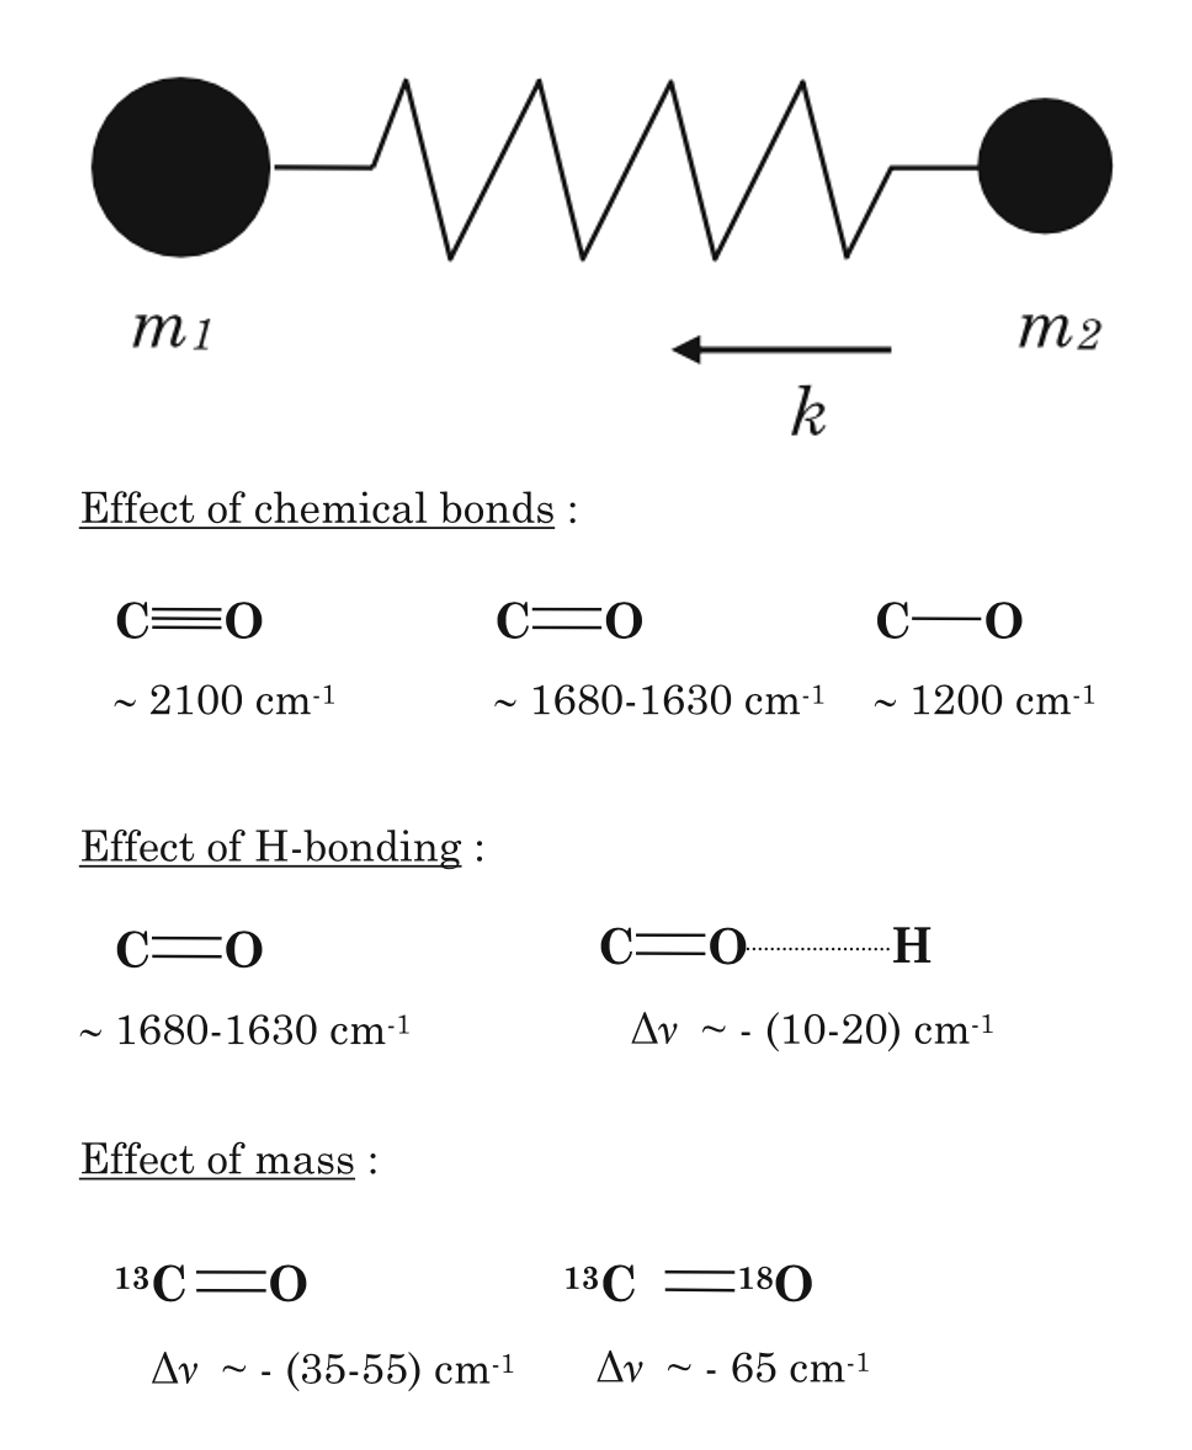
\includegraphics[width=0.8\textwidth]{Images/IR_Basics.png}
  \caption{From \cite{berthomieu_fourier_2009}}
  \label{fig:my-label}
\end{figure}

\begin{figure}[htbp]
  \centering
  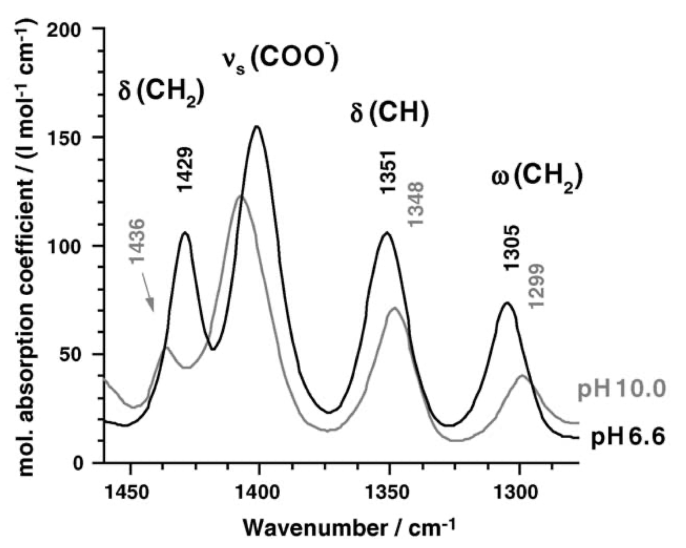
\includegraphics[width=0.8\textwidth]{Images/Cystine_IR_pH_dep.png}
  \caption{From \cite{wolpert_infrared_2006}}
  \label{fig:my-label}
\end{figure}

\begin{figure}[htbp]
  \centering
  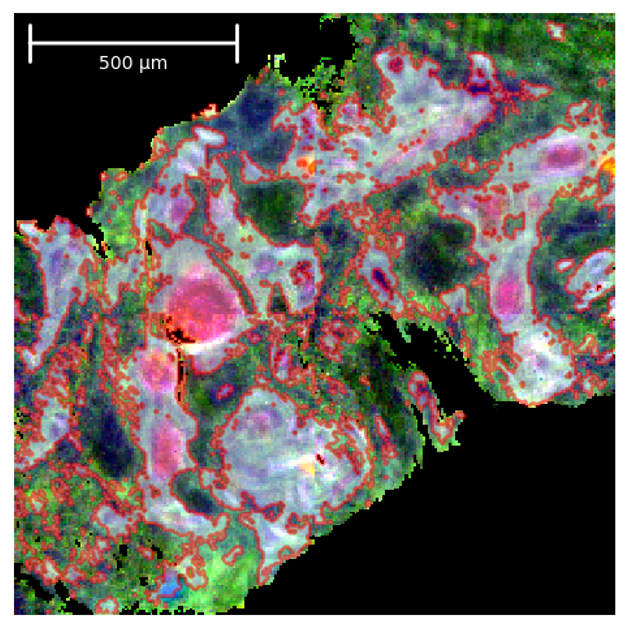
\includegraphics[width=0.8\textwidth]{Images/False_Colour_IR_17.png}
  \caption{Caption}
  \label{fig:my-label}
\end{figure}

\begin{figure}[htbp]
  \centering
  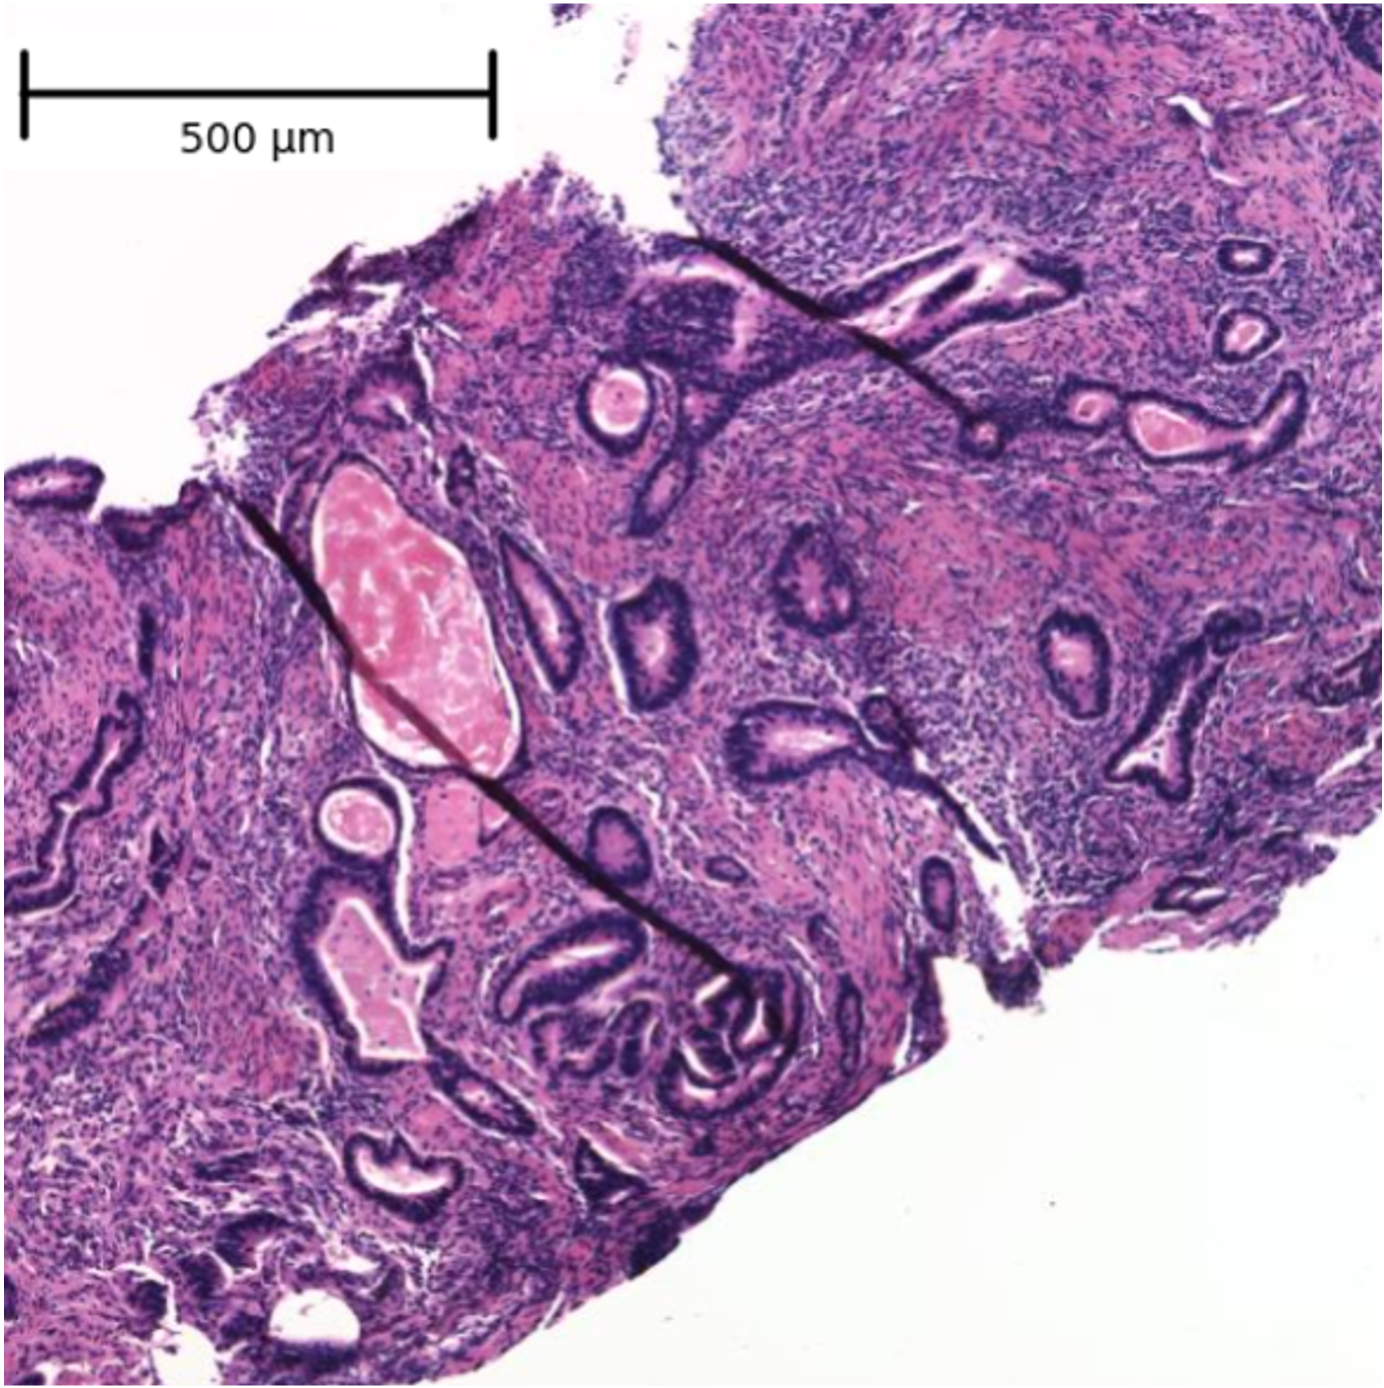
\includegraphics[width=0.8\textwidth]{Images/he_17_scale.png}
  \caption{Caption}
  \label{fig:my-label}
\end{figure}

\begin{figure}[htbp]
  \centering
  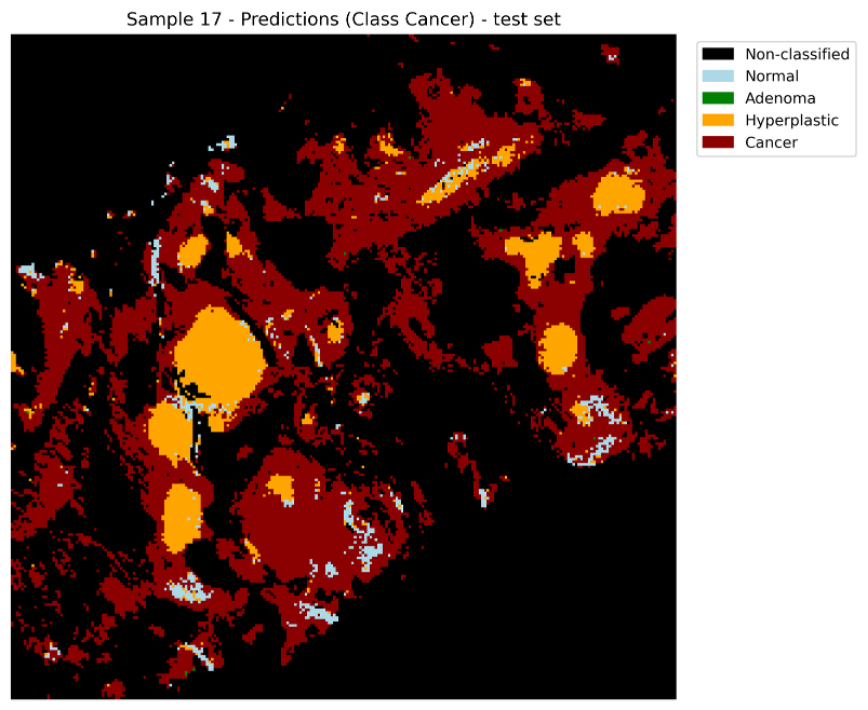
\includegraphics[width=0.8\textwidth]{Images/Predicton_17.png}
  \caption{Caption}
  \label{fig:my-label}
\end{figure}

\subsubsection{Raman Spectroscopy}
\subsubsection{TPEF}
\subsubsection{SHG}

\subsection{Classical ML Methods for Spectral Classification}

\begin{table}[ht] \centering \caption{Sensitivity and specificity (mean ± SD)
for each model.} \label{tab:model_performance} \begin{tabular}{@{}l l c c c c
c@{}} \toprule Model & Metric & Normal & Adenoma & Hyperplastic & Cancer &
Accuracy \\ \midrule \multirow{2}{*}{PCA~$>$~LDA} & Sensitivity & 42 (20.4) & 84
(14.3) & 31 (17.7) & 39 (26.3) & 61 (7.6) \\ & Specificity & 90 (11.1) & 57 (19.
9) & 94 (5.4) & 95 (6.2) & — \\ \midrule \multirow{2}{*}{XGBoost} & Sensitivity
& 58 (11.9) & 80 (14.4) & 41 (14.7) & 62 (33.6) & 68 (10.0) \\ & Specificity &
88 (6.6) & 77 (10.2) & 91 (2.6) & 96 (6.2) & — \\ \midrule \multirow{2}{*}{PCA~$>$~XGBoost} & Sensitivity & 43 (11.5) & 55 (11.9) & 28 (11.9) & 75 (20.9) & 51 (9.
2) \\ & Specificity & 88 (10.3) & 79 (7.7) & 90 (6.7) & 77 (10.5) & — \\
\bottomrule \end{tabular} 
\caption{By Tiago and Pietro}
\end{table} 


% Include the other methods here
\subsubsection{XGBoost}
\subsubsection{Spectral Matching}


\subsection{Deep Learning Methods for Spectral Classification}
\subsubsection{Dataset Challenges}
\begin{figure}[htbp]
  \centering
  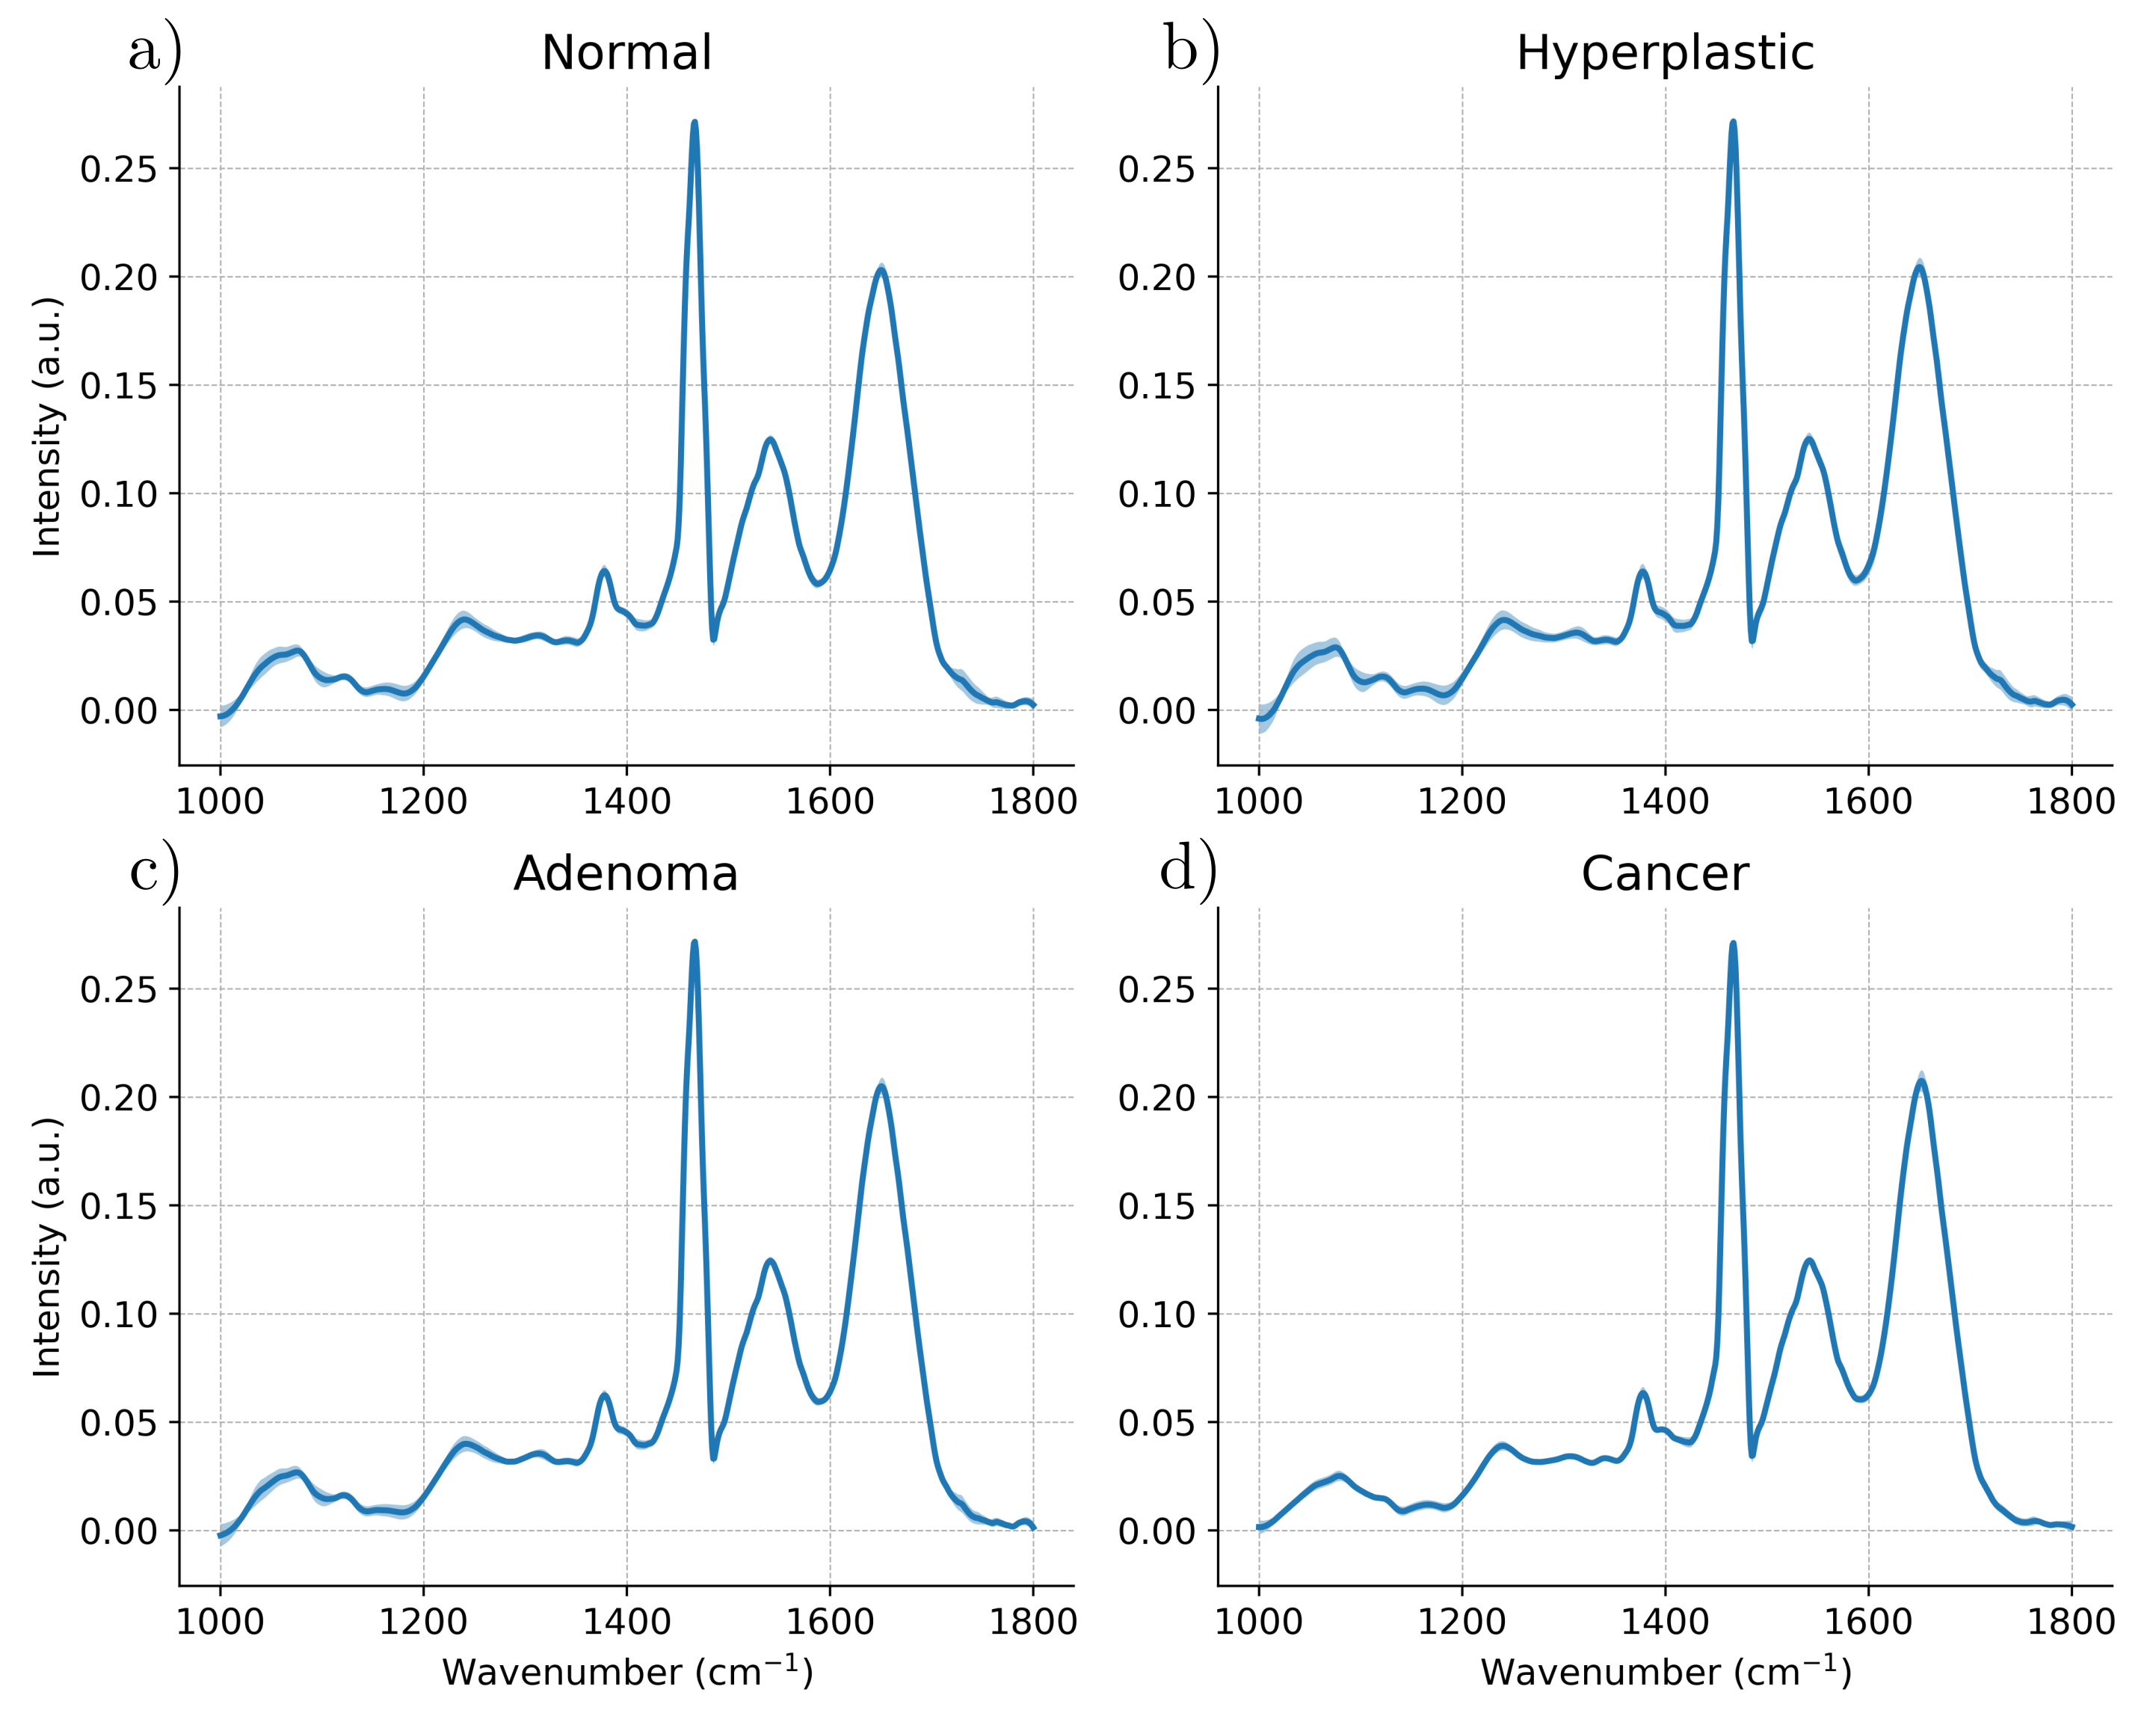
\includegraphics[width=0.8\textwidth]{Images/Dataset_Class_Differences.png}
  \caption{Caption}
  \label{fig:my-label}
\end{figure}

\subsubsection{De-noising Methods}
\subsubsection{Evaluation Metrics}

\subsubsection{Model Architecture}
\begin{figure}[htbp]
  \centering
  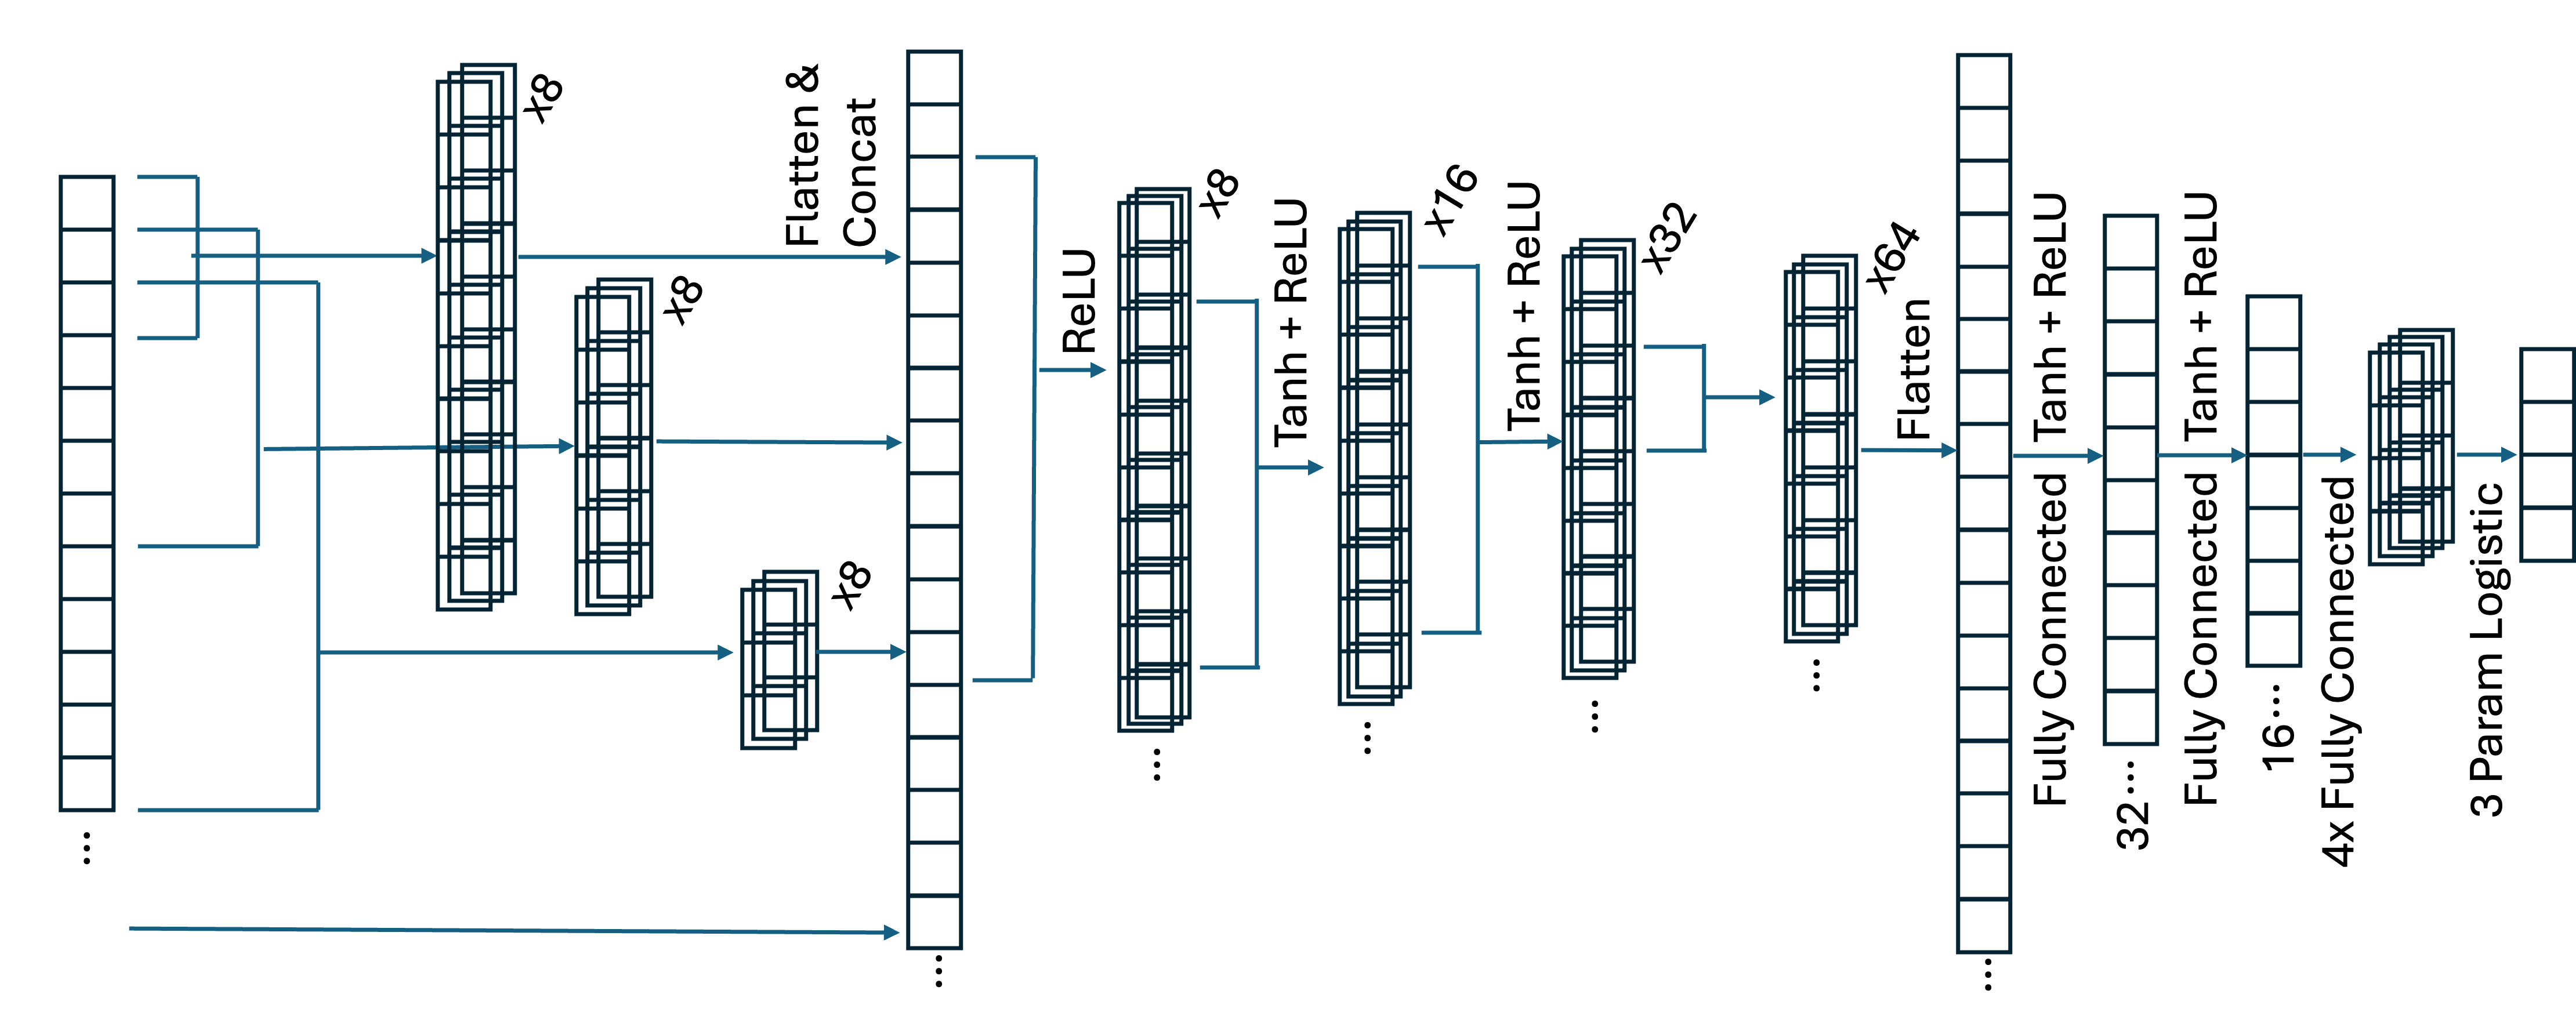
\includegraphics[width=0.8\textwidth]{Images/SCNN_TPL_Arch.png}
  \caption{Caption}
  \label{fig:my-label}
\end{figure}

\begin{figure}[htbp]
  \centering
  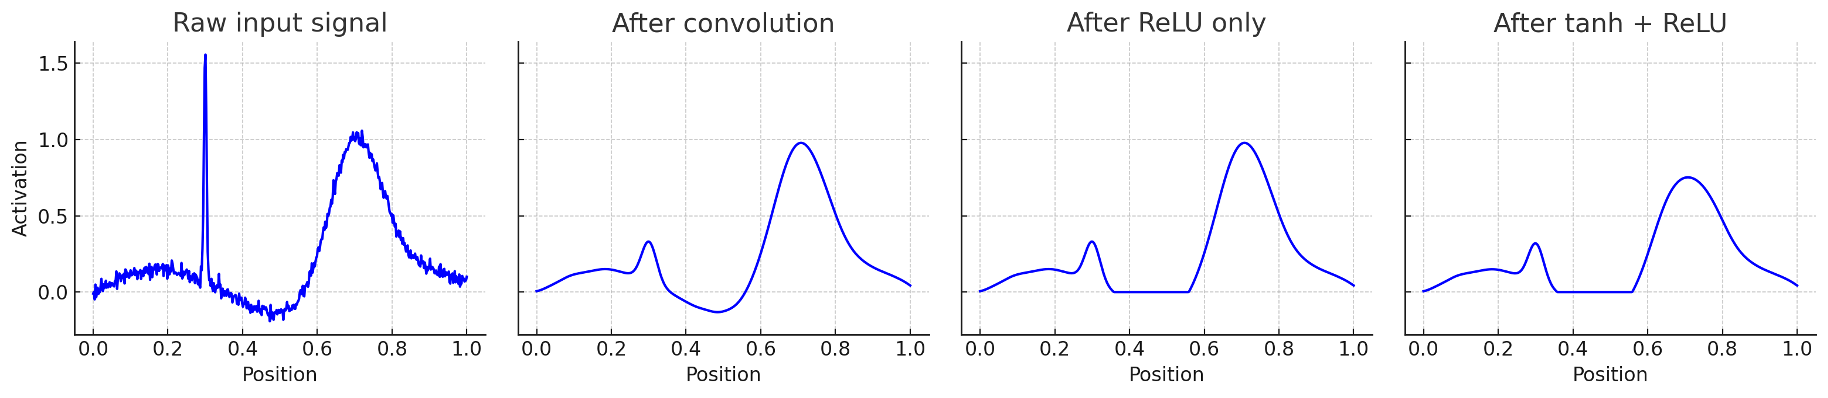
\includegraphics[width=0.8\textwidth]{Images/Tanh_Relu_Demo.png}
  \caption{Caption}
  \label{fig:my-label}
\end{figure}
\subsubsection{Regularisation Techniques}

\begin{figure}[htbp] 
    \centering 
    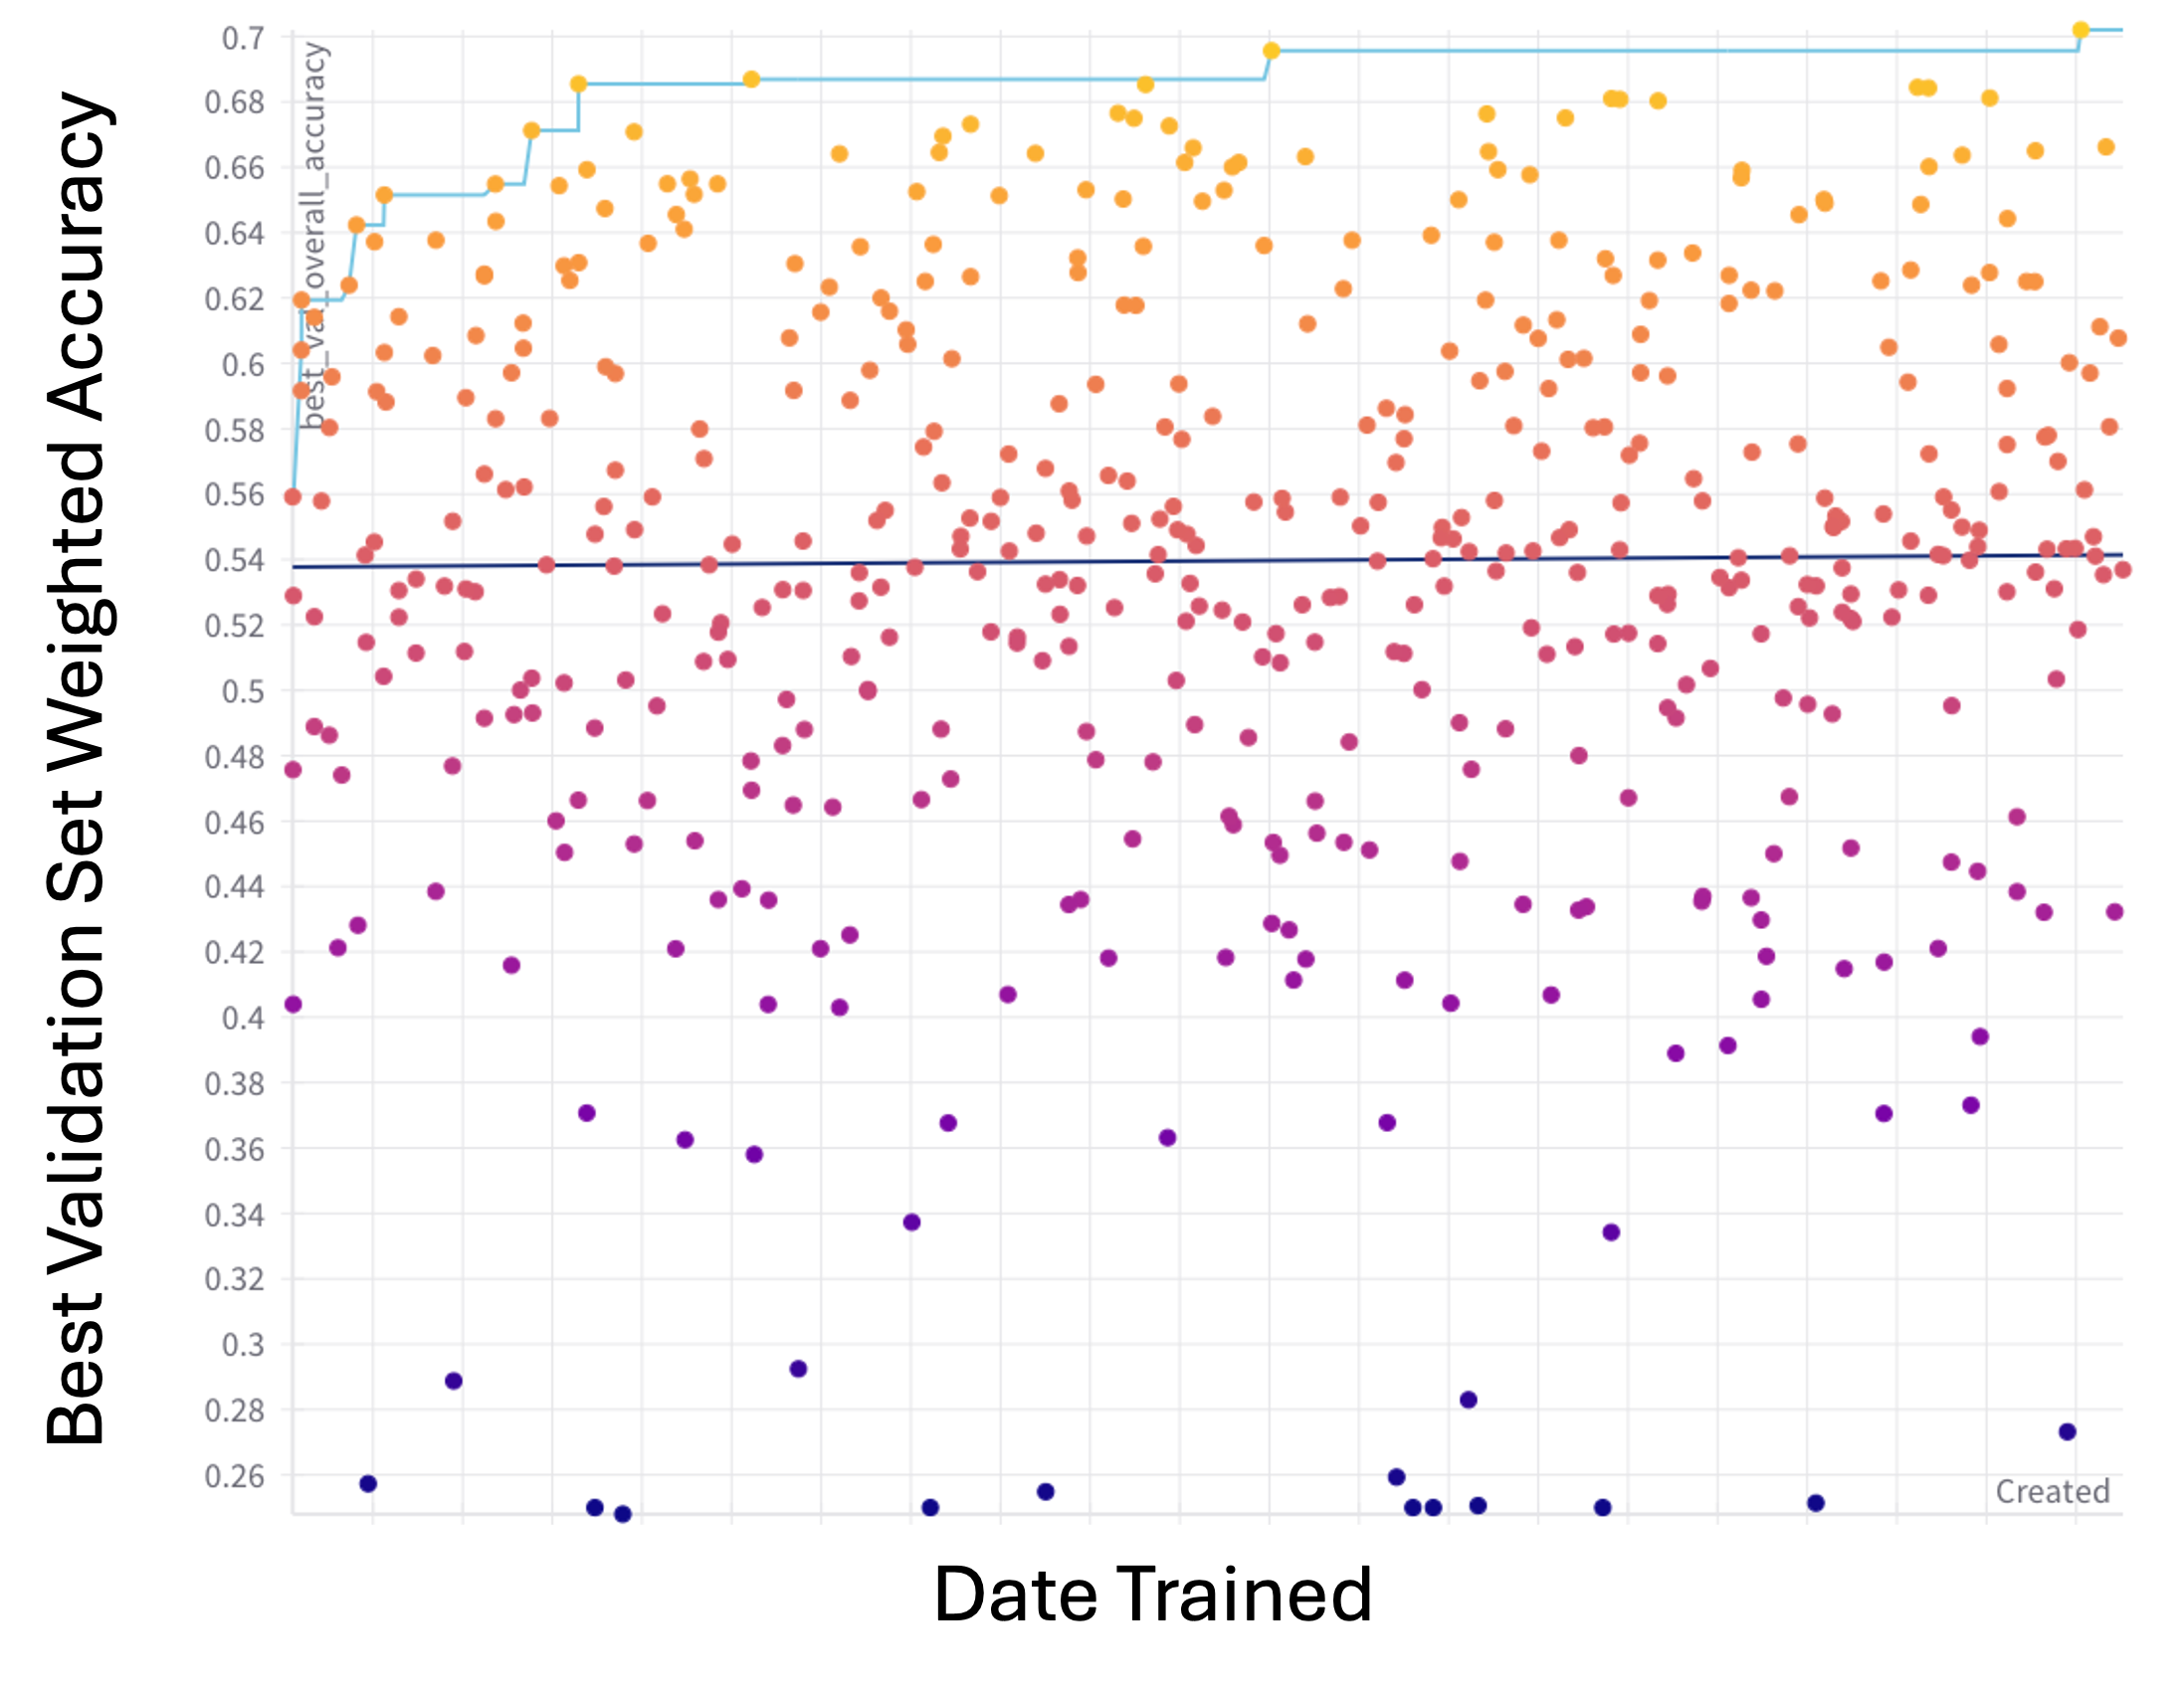
\includegraphics[width=0.8\textwidth]{Images/Ensemble_rough.png} 
    \caption{Caption} \label{fig:my-label}
\end{figure}

\subsection{Explainability}
% A bit of background on why explainability is important and why it must be used in medical contexts
\subsubsection{Local Interpretable Model-Agnostic Explanations}
\subsubsection{CRIME}
\subsubsection{VAE Methods}
\paragraph{Clustering VAE Approaches}
\paragraph{Logic Explained Networks}